% !TEX encoding = UTF-8 Unicode
% !TeX spellcheck = fr_FR
\documentclass[12pt,twoside,a4paper]{article}

% décommenter si nessecaire !TeX TXS-program:compile = txs:///pdflatex/[--shell-escape]
%\usepackage{minted}


\title{Filtre de Kalman}
\author{Sarah Curtit}
\date{}

\usepackage[dvipsnames]{xcolor}
\usepackage{amsfonts}
\usepackage{amsmath}
\usepackage{amssymb}
\usepackage{amsthm}
\usepackage[french]{babel}
\usepackage{beramono}
\usepackage{changepage}
\usepackage{color}
\usepackage{mathdots}
\usepackage[utf8]{inputenc}
\usepackage{enumitem}
\usepackage{fancyhdr}
\usepackage{float}
\usepackage{framed}
\usepackage[T1]{fontenc}
\usepackage[margin=1in]{geometry}
\usepackage{listings}
\usepackage{mathrsfs}
\usepackage{tikz, tkz-tab}
\usepackage[european resistor]{circuitikz}
\usepackage{titling}
\usepackage{tabularx}
\usepackage{graphicx}
\usepackage{textcomp}
\usepackage{gensymb} %en tant que le package 'was'
\usepackage{physics}
\usepackage{marvosym}
\usepackage{standalone}
\usepackage{preview}
\usepackage{mathtools}
\usepackage[hidelinks]{hyperref}
\hypersetup{allcolors=black}


\usetikzlibrary{decorations.pathmorphing,patterns}

\newtheoremstyle{dotless}{}{}{\itshape}{}{\bfseries}{}{ }{}
\theoremstyle{dotless}

\newtheorem{defs}{D\'efinition}[subsection]
\newenvironment{defi}{\definecolor{shadecolor}{RGB}{255,236,217}\begin{shaded}\begin{defs}\ \\}{\end{defs}\end{shaded}}

\newtheorem{pro}{Propri\'et\'e}[subsection]
\newenvironment{prop}{\definecolor{shadecolor}{RGB}{230,230,255}\begin{shaded}\begin{pro}\ \\}{\end{pro}\end{shaded}}

\newtheorem*{theos}{Th\'eor\`eme}
\newenvironment{theo}[1]{\definecolor{shadecolor}{RGB}{230,230,255}\begin{shaded}\begin{theos}\textbf{\emph{#1}}\ \\}{\end{theos}\end{shaded}}

\newtheorem{cor}{Corollaire}[subsection]
\newenvironment{coro}{\definecolor{shadecolor}{RGB}{245,250,255}\begin{shaded}\begin{cor}\ \\}{\end{cor}\end{shaded}}

\setlength{\droptitle}{-1in}
%\predate{}
%\postdate{}
%\title{\textbf{\titre}\\\soustitre\vspace{-.18in}}

\pagestyle{fancy}
\makeatletter
\lhead{\title}
\rhead{\@author}
\makeatother

\newenvironment{preuve}{\begin{framed}\begin{proof}[\unskip\nopunct]}{\end{proof}\end{framed}}
\newenvironment{liste}{\begin{itemize}[leftmargin=*,noitemsep, topsep=0pt]}{\end{itemize}}
\newenvironment{tab}{\begin{adjustwidth}{.5cm}{}}{\end{adjustwidth}}

\newcommand{\lbracket}{[\![}
\newcommand{\rbracket}{]\!]}
\newcommand{\fonction}[5]{\begin{aligned}[t]#1\colon#2&\longrightarrow#3 \\#4&\longmapsto#5\end{aligned}}
\newcommand{\systeme}[1]{\left\{\begin{aligned}#1\end{aligned}\right.}
\newcommand{\cercle}[1]{\textcircled{\scriptsize{#1}}}
\newcommand{\Sup}{\mathop{\text{Sup}}}
\newcommand{\Inf}{\mathop{\text{Inf}}}
\newcommand{\lf}[1]{\left(#1\right)}
%\newcommand{\C}{\mathbb{C}}
\newcommand{\R}{\mathbb{R}}
\newcommand{\K}{\mathbb{K}}
\newcommand{\Q}{\mathbb{Q}}
\newcommand{\N}{\mathbb{N}}
\newcommand{\Z}{\mathbb{Z}}
\newcommand{\I}{\mathcal{I}}
\newcommand{\F}{\mathcal{F}}
\newcommand{\E}{\mathcal{E}}
%\newcommand{\G}{\mathcal{G}}
\newcommand{\et}{\text{ et }}
\newcommand{\ou}{\text{ ou }}
\newcommand{\xou}{\ \fbox{\text{ou}}\ }
\newcommand{\vdashv}{\mathrel{\text{\ooalign{$\vdash$\cr$\dashv$\cr}}}}
\newcommand{\card}{\text{card}}
\newcommand{\restr}[2]{{% we make the whole thing an ordinary symbol
		\left.\kern-\nulldelimiterspace % automatically resize the bar with \right
		#1 % the function
		\vphantom{\big|} % pretend it's a little taller at normal size
		\right|_{#2} % this is the delimiter
	}}
\newcommand{\floor}[1]{\lfloor #1 \rfloor}
\newcommand{\ceil}[1]{\lceil #1 \rceil}
\newcommand{\Sev}{\mathrm{S}_\mathrm{EV}}
\newcommand{\vect}{\mathrm{Vect}}
\newcommand{\Kev}{\K_\mathrm{EV}}

%%
%% Julia definition (c) 2014 Jubobs
%%
\lstdefinelanguage{Julia}%
{
	morekeywords={abstract,break,case,catch,const,continue,do,else,elseif,%
		end,export,false,for,function,immutable,import,importall,if,in,%
		macro,module,otherwise,quote,return,switch,true,try,type,typealias,%
		using,while},%
	sensitive=false,%
	alsoother={$},%
	morecomment=[l]\#,%
	morecomment=[n]{\#=}{=\#},%
	morestring=[s]{"}{"},%
	morestring=[m]{'}{'},%
}[keywords,comments,strings]%

%%
%% Laplacien et D'Alembertien
%%
\newcommand*\Laplace{\mathop{}\!\mathbin\bigtriangleup}
\newcommand*\DAlambert{\mathop{}\!\mathbin\Box}

\usepackage[utf8]{inputenc}

\newcommand\ul[1]{\underline{#1}}
\newcommand\ull[1]{\underline{\underline{#1}}}
%\usepackage{minted}

\newenvironment{changemargin}[2]{\begin{list}{}{%
\setlength{\topsep}{0pt}%
\setlength{\leftmargin}{0pt}%
\setlength{\rightmargin}{0pt}%
\setlength{\listparindent}{\parindent}%
\setlength{\itemindent}{\parindent}%
\setlength{\parsep}{0pt plus 1pt}%
\addtolength{\leftmargin}{#1}%
\addtolength{\rightmargin}{#2}%
}\item }{\end{list}}



\begin{document}
	\maketitle
	
\section{Presentation du Filtre de Kalman}

\subsection{Le filtre de Kalman continu}

\subsubsection{Le modèle}
	
Le filtre de Kalman est un modèle d'état défini par deux équations: 

$$
\left\{ 
\begin{array}{ll}
        \dot{x}(t) = A x(t)  + B u(t) +M w(t)  & \text{équation d'état}  \\
        y(t) = C x(t) + Du(t) + v(t) & \text{équation de mesure} 
\end{array}
\right.
$$



x est un vecteur d'état, y un vecteur de mesures, u un vecteur de commandes (données déterminées), tandis que les signaux $w(k)$ et $v(k)$ sont des bruits blancs gaussiens centrés de densité spectrale de puissance $W$ et $V$ respectivement. On a 
$$
\begin{array}{lll}
E[w(k) w(k+l)^T ] &= W\delta(l) & \delta(l) \text{ = 1 si l=0; 0 sinon} \\
E[v(k) v(k+l)^T ] &= V \delta(l) & \text{(V doit être inversible)}\\
E[w(k) v(k+l)^T ] &= 0 & \\
\end{array}
$$

\subsubsection{Minimisation de l'erreur d'estimation} 

En pratique, le filtre doit retourner en sortie l'état estimé du système, noté $\hat{x}$.
L'équation d'état du filtre nous est donnée par 
$$ \hat{\dot{x}}(t) = A_f\hat{x}(t)+B_fu(t)+K_fy(t) $$
où $A_f$ $B_f$ et $K_f$ sont des matrices à déterminer. \\
\vspace{0.5cm}

\noindent Soit $\varepsilon(t)= x(t)-\hat x(t)$ l'erreur d'estimation du système. On souhaite que cet estimateur soit non biaisé, c'est à dire que $\lim\limits_{t \rightarrow +\infty } \bar{\varepsilon}= 0 $ quel que soit le profil de commande et quel que soit l'état initial ($\bar{\varepsilon}$ étant l'espérance mathématique de $\varepsilon$). 
\vspace{0.5cm}\\
L'écriture de ces conditions nous donne finalement l'équation du filtre de Kalman 
$$
\hat{\dot{x}}(t) = (A\hat x + Bu) + K_f (y -C \hat x -Du)
$$
$K_f$ est appelé le gain du filtre. C'est lui qui traduit la confiance que l'on a dans le modèle ou les mesures. Si on considère que le modèle est très fiable et les mesures très bruitées on accordera peu d'importance à celles-ci, et $K_f$ sera petit. Si l'on fait au contraire plus confiance aux mesures qu'au modèle, $K_f$ sera grand. 
\vspace{1cm}

Afin d'obtenir le filtre le plus fiable possible, le gain $K_f$ doit minimiser la variance de l'erreur d'estimation, c'est à dire la trace de la matrice de covariance de l'erreur d'estimation, 
$$
\begin{array}{lll}
P(t) &=& E[(x(t)-\hat x(t))(x(t)-\hat x(t))^T] \\
\end{array}
$$ 

$P(t)$ vérifiant l'équation
$$ 
\dot{P}(t) = (A-K_{f}C)P(t)+P(t)(A-K_{f}C)^{T} + MWM^{T} + K_{f}VK_{f}^{T}
$$

En minimisant P on obtient
$$
\begin{array}{lll}
K_f &=& P(t)C^T V^{-1} \\
\dot{P}(t) &= &AP(t) +P(t)A^T -P(t)C^TV^{-1}CP(t)+MWM^T
\end{array}
$$

Cette deuxième équation étant appelée équation différentielle de Riccati.
\vspace{1cm}

Une fois les erreurs d'initialisation corrigées (régime constant), on obtient 
$$
\begin{array}{llll}
K_f &=& P(t)C^T V^{-1} &\text{Désormais constant.}\\ 
0 &= &AP(t) +P(t)A^T -P(t)C^TV^{-1}CP(t)+MWM^T & \text{P étant la solution positive de l'équation.}
\rule[0pt]{0mm}{15pt} \\
\end{array}
$$



\subsection{Le filtre de Kalman discret}

\subsubsection{Le modèle}
Dans les faits, les appareils numériques fonctionnent de manière discrète. \\
On utilisera donc en pratique le modèle de Kalman discret
$$
\left\{ 
\begin{array}{lll}
        x(k+1) = A_d x(k) + B_d u(k) +M_d w_d(k) & \text{équation d'état} & x \in \mathbb{R}^n, y \in \mathbb{R}^m, w_d \in \mathbb{R}^q\\
       y(k) = C_d x(k) + Du(k) + v_d(k) & \text{équation de mesure} & y \in \mathbb{R}^m, v_d \in \mathbb{R}^p\\
\end{array}
\right.
$$

Les signaux $w_d$ et $v_d$ sont cette fois associés à des matrices de covariance $W_d$ et $V_d$ telles que
$$
\begin{array}{lll}
E[w_d(k) w_d(k+l)^T ] &= W_d \delta(l) &  \\
E[v_d(k) v_d(k+l)^T ] &= V_d \delta(l) & \text{($V_d$ doit être inversible)}\\
E[w_d(k) v_d(k+l)^T ] &= 0 & \\
\end{array}
$$
On note $dt$ le pas de temps associé au système discret.\\

\subsubsection{Passage du modèle continu au modèle discret}

\vspace{0.3cm}
Le modèle de Kalman discret est très proche du modèle continu, et on peut obtenir les nouvelles matrices discrètes à partir de celles du modèle continu. On a
$$ \begin{array}{ccccc}
A_d = e^{Adt} \rule[0pt]{30pt}{0pt}
B_d = \int_0^{dt} e^{Av}B \, \mathrm{d}v \rule[0pt]{30pt}{0pt}& 
M_d = I_n \rule[0pt]{30pt}{0pt}&
C_d = C\rule[0pt]{30pt}{0pt} & 
V_d= \frac{V}{dt}\rule[0pt]{30pt}{0pt}\\
\end{array} $$

\noindent L'expression de $W_d$ est plus compliquée puisqu'on a $W_d = \int_0^{dt}e^{Av}MWM^Te^{A^T v} \, \mathrm{d}v$ \\
Cependant dans l'hypothèse où $dt$ est petit par rapport au temps de réponse du système, on peut écrire
$$ W_d \approx dtMWM^T$$ 

\subsubsection{Représentation d'état, implémentation du filtre en pratique}


Comme dans le modèle continu, on souhaite optimiser le gain $K_{f}$ afin de minimiser l'erreur d'estimation. \\
Dans la suite de cette section, on distinguera 
$$
\begin{array}{ll}
	\begin{array}[t]{l}
	\text{l'état prédit à l'instant k+1}\\
	\text{connaissant toutes les mesures jusqu'à l'instant k} 
	\end{array} & \hat x(k+1|k) \\
	
	\begin{array}{l}
	\text{l'état estimé connaissant la mesure à l'instant k+1 (après recalage)} 
	\end{array} & \hat x(k+1|k+1) \rule{0pt}{15pt}
\end{array}
$$ 

\noindent L'état prédit est calculé de fa\c con déterministe
$$ \hat x(k+1|k) = A_{d} \hat x (k|k) +B_du(k)$$

\noindent Tandis que l'équation d'état du filtre 
$$ \hat{\dot{x}}(k|k) = A_d\hat{x}(k|k)+B_du(k)+K_f(k+1)\big(y(k) - C_{d} \hat x(k|k) - D \hat x(k|k) \big) $$
\indent nous donne 
$$ \hat x(k+1|k+1) = \hat x(k+1|k)+ K_{f}(k+1)\big(y(k) - C_{d} \hat x(k|k) - D \hat x(k|k) \big)$$

La combinaison de ces deux équations nous permet d'obtenir la représentation d'état du filtre de Kalman permanent: 
$$
\boxed{
\left\{
\begin{array}{lll}
\hat x(k|k) &=& (I-K_f C_d)\hat x(k|k-1)+
	\begin{pmatrix} K_f & -K_f D \end{pmatrix}
	\begin{pmatrix} y(k) \\ u(k) \end{pmatrix} \\
\hat x( k+1|k) &=& A_d(I-K_f C_d) \hat x (k|k-1) + 
	\begin{pmatrix} A_d K_f & B_d-A_dK_fD \end{pmatrix}
	\begin{pmatrix} y(k) \\ u(k)\end{pmatrix} \\
\end{array}
\right.}
$$

\noindent C'est la deuxième équation, calculant l'état prédit à l'instant k+1 qui nous intéresse et qui sera implémenté dans l'algorythme du filtre de Kalman. \\

\vspace{1cm} 

Afin de totalement déterminer cette équation, il reste cependant à déterminer $K_{f}$, choisi encore une fois afin de minimiser l'erreur d'estimation $P(k+1|k+1)$ (dont l'expression est extrêmement compliquée).

La résolution de l'équation différentielle nous donne 
$$
\begin{array}{lll}
K_{f}(k+1) &=& P(k+1|k)C_{d}^{T}(C_{d}P(k+1|k)C_{d}^{T}+V_{d})^{-1} \\
P(k+1|k) &=&  A_{d}P(k|k-1)A_{d}^{T} -A_{d}P(k|k-1)C_{d}^{T}\big(C_{d}P(k|k-1)C_{d}^{T}+V_{d}\big)^{-1}C_{d}P(k|k-1)A_{d}^{T} \\
&& + M_{d}W_{d}M_{d}^{T}
\end{array}
$$

En régime permanent la matrice de covariance de l'erreur de prédiction est constante et vérifie l'équation discrète de Riccati
$$ P_{p} =  A_{d}P_{p}A_{d}^{T} -A_{d}P_{p}C_{d}^{T}\big(C_{d}P_{p}C_{d}^{T}+V_{d}\big)^{-1}C_{d}P_{p}A_{d}^{T}  + M_{d}W_{d}M_{d}^{T} $$

\vspace{1cm} 
On peut en déduire le gain du filtre et la matrice de covariance de l'erreur d'estimation 
$$ 
\begin{array}{lll}
K_{f} &=& P_{p}C_{d}^{T}(C_{d}P_{p}C_{d}^{T}+V_{d})^{-1} \\
P_{e} &=& (I-K_{f}C_{d})P_{p}
\end{array}$$



La plupart des solveurs actuels proposent des fonctions permettant de résoudre l'équation de Riccati. 
Dans le cadre de ce projet, nous avons travaillé avec Python et la fonction scipy.linalg.solve\_discrete\_are. \\

\section{Application au problème}

On souhaite asservir en effort un robot 6 axes. L'objectif est d'appliquer une force choisie (constante ou non) le long d'une trajectoire parcourant une surface irrégulière. Un capteur 6 axe fixé au bout du bras du robot nous indique les forces et moments appliqués par l'outil (un poussoir à bille) sur le capteur. \\
Afin d'effectuer la tâche demandée, nous définissons une trajectoire de base censée suivre la forme de la surface. L'outil supporté par le robot est censé tourner avec la surface pour rester en permanence normal à celle-ci. Nous fonctionnerons dans la suite dans le repère du Tool Center Point.\\
 Avant de démarrer, nous descendons lentement le robot à la verticale du point de départ jusqu'à ce que le capteur mesure la force désirée (selon z donc). Nous démarrons ensuite la trajectoire que nous corrigeons au fur et à mesure en fonction des données renvoyées par le capteur afin de rester en permanence le plus proche possible de la force objectif. Nous pensions à l'origine utiliser un filtre de Kalman, mais la rigidité du robot devant le poussoir à bille (de raideur 3.1 N/mm) entraîne plusieurs problèmes: nous ne pouvons plus écrire de modèle dynamique et les erreurs sur la position du robot et les aspérités de la surface deviennent en apparence impossible à intégrer correctement au problème. Nous sommes donc dans l'impossibilité de définir mathématiquement le gain du Filtre.


\subsection{Problème 1D}

Pour simplifier le problème, considérons tout d'abord que l'outil utilisé est parfaitement perpendiculaire à la surface au point de contact et qu'il n'y a pas de frottement. Dans ce cas, on peut se permettre de considérer seulement les données selon z (repère orienté selon la normale à la surface au point courant).

On prend alors comme vecteurs d'état, de mesure et de commande respectivement
$$
\begin{array}{ccc}
x =  \begin{pmatrix} z & \dot{z} \end{pmatrix} 
,   & 
y= \begin{pmatrix}
 F_z \
\end{pmatrix},   &
u = \begin{pmatrix} \dot{z}_{robot} \\ F_{obj}\end{pmatrix} \\
\end{array}
$$

ce qui simplifie grandement le problème

\subsubsection{Détermination des données du problème dans le cas continu}


v et w sont ici respectivement le vecteur des signaux aléatoires qui polluent les mesures y et le vecteur  des signaux inconnus qui viennent perturber directement l'équation d'état du système. Ici  v représente l'imprécision du capteur et w rend compte des aspérités de la surface et de l'imprécision du robot. \\
La matrice M relie le bruit d'état $w_x$ à w par la relation $w_x = Mw$ \\
\vspace {1cm} \\
En faisant pour l'instant abstraction des vecteurs d'erreurs (et donc du dernier terme de chaque égalité) le système s'écrit dans notre cas comme  

$$
\left\{ 
\begin{array}{ll}
        \begin{pmatrix} \dot{z} \\ \ddot{z} \end{pmatrix} 
        &= \begin{pmatrix}
        0 & 1 \\
        0 & 0 \\ 
        \end{pmatrix}.
        \begin{pmatrix} z  \\ \dot{z} \end{pmatrix} \\
        \vspace{0.5cm} \\
        \begin{pmatrix} F_z  \end{pmatrix}
         &= \begin{pmatrix} k & 0 \end{pmatrix}.
	 	\begin{pmatrix} z \\  \dot{z} \end{pmatrix} 
	+ \begin{pmatrix} 0 & 1 \end{pmatrix}
	 \begin{pmatrix} \dot{z}_{robot} \\ F_{obj}\end{pmatrix}\\
\end{array}
\right.
$$

Le choix a été fait ici de considérer l'accélération comme nulle car le déplacement du bras du robot est commandé en fonction de la force exercée sur le ressort, il n'en dépend pas directement. --> \textcolor{red}{Premier problème : le système n'est en fait pas dynamique.}
\\
La matrice C est elle déterminée à partir d'une simple loi de Hooke: $F_z = -k*d_z$. 

\vspace{2cm}

Déterminons désormais les  matrices associées vecteurs d'erreur v et w. \\
on note 
$$
\begin{array}{lll}
 v &= \begin{pmatrix}  v_{F_{z}}  \end{pmatrix} ^T  & \text{où $v_{F_{z}}$ représente l'incertitude sur la mesure $F_z$ du capteur} \\
 w &= \begin{pmatrix} w_z  \end{pmatrix}&
 		\text{où}
		\begin{array}[t]{l}
		\text{$w_z$ représente l'incertitude de position du robot selon z} \\
		\end{array} \\
 \end{array}
 $$
 
% Pour ce qui est du vecteur v son unique composante comprend en fait 3 termes associés respectivement 
% $$
% \begin{array}{l}
% 	\text{à l'incertitude de mesure du capteur} \\
%	\text{à l'incertitude sur les aspérités de la surface} \\
%	\text{à l'incertitude sur la position du robot}
% \end{array}
% $$
% 
% Bien que ces deux dernières contributions soient intuitivement per comme des bruits d'état, elle ne viennent en fait pas perturber directement la vitesse ou l'accélération du robot, perçu comme infiniment rigide devant le poussoir à bille. Elle viennent cependant comprimer plus ou moins le ressort du poussoir et donc modifier les données reçues par le capteur. \\

\textcolor{red}{Deux sources supplémentaires d'erreur sont l'incertitude sur la position du robot et l'incertitude sur les aspérités de la surface. Problème: comment les prendre en compte ? Intuitivement il s'agit de d'erreurs liées à l'état du système, cependant le système n'est pas dynamique et elles ne viennent pas s'insérer dans l'équation. Si on les compte comme des contributions à l'erreur de mesure l'erreur de mesure sera disproportionnée devant l'erreur d'état (notamment à cause des aspérités de surface). }
 
 \vspace{0.5cm}


w(t) et v(t) sont des vecteurs gaussiens centrés de densité spectrale de puissance W et V respectivement. On a :

$$
\begin{array}{ll}
E[w(t) w(t+\tau)^T ] &= W \delta(\tau) \\
E[v(t) v(t+\tau)^T ] &= V \delta(\tau)  \\
E[w(t) v(t+\tau)^T ] &= 0  \\
\end{array}
$$

\vspace{1cm}

V peut-être calculé à partir des données d'échantillonnage du capteur. Le certificat d'étalonnage nous indique en effet les précisions suivantes:
$$
\begin{array}{|c|c|c|c|c|c|}	
	\hline
	\bold{\delta F_x} & \bold{\delta F_y} & \bold{\delta F_z} & \bold{\delta M_x} & \bold{\delta M_y} & \bold{\delta M_z} \\
	\hline 
	1.00\% & 1.25\% & 0.75\% & 1.00\% & 1.25\% & 1.50\% \\
	\hline
\end{array}
$$

On estime également les ordres de grandeur des forces et moments qui seront rencontrés par le capteur (avec les hypothèses émises précédemment)
$$
\begin{array}{|c|c|c|c|c|c|}	
	\hline
	\bold{\bar{F}_x} & \bold{\bar{F}_y} & \bold{\bar{F}_z} & \bold{\bar{M}_x} & \bold{\bar{M}_y} & \bold{\bar{M}_z} \\
	\hline 
	0N & 0N & 20N & 0N.m & 0N.m & 0N.m \\
	\hline
\end{array}
$$

La précision du robot et des aspérités de la surface sont 
$$
\begin{array}{|c|c|}
\hline 
\bold{\delta z_{robot}} & \bold{\delta z_{asp}} \\
\hline 
0.02mm & 1mm \\
\hline
\end{array}
$$

L'ordre de grandeur des aspérités représente ici la différence de hauteur de surface non prévue maximale qui puisse être rencontrée entre deux pas de temps.\\

\vspace{1cm}
V est la matrice de densité spectrale de puissance du vecteur $\ul{v}$. Chaque source d'erreur étant indépendante, cela signifie que la matrice est diagonale, et on a 
$$ 
\begin{array}{ll}
V_{ii} &= \mathcal{L}[\phi_{ii}(\tau)] \\
&= \int_{-\infty}{+\infty} E[v_{i}(t)v_{i}(t+\tau)^{t}] \, \mathrm{d}\tau
\end{array}
$$

Le vecteur v étant un bruit blanc gaussien centré, les choses se simplifient. En effet on a $\forall v_{i}$
$$\phi(t,\tau)_{ii} = \sigma_{i}^{2}\delta(0)$$ et donc
$$V_{ii} = \sigma_{i}^{2} = Var(v_{i})$$

Il ne reste plus qu'à calculer les écarts types associés à chaque erreur. L'intervalle de confiance à 95\% étant l'intervalle $[m-1.96\sigma, m+1.96\sigma]$ (m étant la moyenne) on a 
$$
\begin{array}{lrcl}
	&\text{[}-\delta F_{z}*\bar{F}_{z} \rule{2mm}{0mm} ; \rule{2mm}{0mm} \delta F_{z}*\bar{F}_{z} \text{]} &=& \text{[} -1.96*\sigma_{F_{z}} \rule{2mm}{0pt}; \rule{2mm}{0pt}1.96*\sigma_{F_{z}}  \text{]} \\
%	&\text{[} -k*\delta z_{asp} \rule{2mm}{0pt}; \rule{2mm}{0pt} k*\delta z_{asp} \text{]} &=& \text{[}-1.96*\sigma_{k*z_{asp}} \rule{2mm}{0pt}; \rule{2mm}{0pt}1.96*\sigma_{k*z_{asp}}  \text{]} \\
%	&\text{[} -k*\delta z_{robot} \rule{2mm}{0pt}; \rule{2mm}{0pt} k*\delta z_{robot} \text{]} &=& \text{[}-1.96*\sigma_{k*z_{robot}} \rule{2mm}{0pt}; \rule{2mm}{0pt}1.96*\sigma_{k*z_{robot}}  \text{]} \\
	\text{Soit} & & & \\
	& \sigma_{F_{z}} &=&  \frac{\delta F_{z}*\bar{F}_{z}}{1.96} \\
%	& \sigma_{k*z_{asp}} &= & \frac{k*\delta z_{asp}}{1.96}  \rule{0pt}{15pt}\\
%	&\sigma_{k*z_{robot}} &= & \frac{k*\delta z_{robot}}{1.96}  \rule{0pt}{15pt}\\
\end{array}
$$

\vspace{1cm}
On en déduit
$$
\begin{array}{ll}
V &= \begin{pmatrix}
\sigma_{F_{z}}^{2} %+  \sigma_{z_{asp}}^{2} +  \sigma_{z_{robot}}^{2} 
\end{pmatrix} \\
&=  \begin{pmatrix}
\frac{(\delta F_{z}*\bar{F}_{z})^{2}}{1.96^{2}}%+(k\delta z_{asp})^{2}+(*\delta z_{robot})^{2}
\end{pmatrix} \rule{0pt}{20pt} \\
%&= \begin{pmatrix} 2.607 \end{pmatrix} \rule{0pt}{20pt}
&= \begin{pmatrix} 5.857*10^{-3} \end{pmatrix} \rule{0pt}{20pt}
\end{array}
$$

On remarque ici que la contribution de l'imprécision du robot à la matrice V est négligeable (de l'ordre de $10^{-8}$) devant l'imprécision du capteur. Le robot est en effet extrêmement précis. La contribution des aspérités de surfaces est également ici négligeable, mais il serait envisageable d'augmenter l'ordre de grandeur de ces aspérités si notre système est efficace.  



\vspace{2cm}

W est ensuite calculé de la même façon, en considérant que $\delta \dot{z}_{robot} = \delta z_{robot} = 0.02mm$

$$
\begin{array}{rcl}
	\text{[} -\delta \dot{z}_{robot} \rule{2mm}{0pt}; \rule{2mm}{0pt} \delta \dot{z}_{robot} \text{]} &=& \text{[}-1.96*\sigma_{dot{z}_{robot}} \rule{2mm}{0pt}; \rule{2mm}{0pt} 1.96*\sigma_{\dot{z}_{robot}}  \text{]} \\
	\sigma_{\dot{z}_{robot}} &= & \frac{\delta\dot{z}_{robot}}{1.96} \rule{0pt}{15pt} \\
\end{array}
$$

$$
\begin{array}{ll}
W &=
\begin{pmatrix}
 \sigma_{\dot{z}_{robot}}^{2} 
\end{pmatrix} \\
&=
\begin{pmatrix}
(\frac{\delta\dot{z}_{robot}}{1.96})^{2}
\end{pmatrix} \rule{0pt}{20pt} \\ 
&= \begin{pmatrix} 1.041*10^{-8} \end{pmatrix} \rule{0pt}{20pt} \\ 
\end{array}
$$

\vspace{0.5cm}

Déterminons enfin la matrice M qui permet de "relier" le vecteur w à l'équation d'état. Elle est ici triviale puisqu'on a tout simplement 
$$
M = 
\begin{pmatrix}
1 \\ 0
\end{pmatrix}
$$


\vspace{0.5cm}

Toutes les données de l'équation ayant été définies, on peut désormais calculer les matrices associées au modèle discret
\begin{changemargin}{-1.5cm}{0cm}
$$
\begin{array}{ccc}
    \begin{array}[t]{rcl}
    A_{d} &=& e^{Adt} \\
    &=&e^{\begin{pmatrix} 0 & dt \\ 0 & 0 \end{pmatrix}}\\
    &= & \begin{pmatrix} 1 & 0 \\ 0 & 1 \end{pmatrix} + \begin{pmatrix} 0 & dt \\ 0 & 0 \end{pmatrix}+ \begin{pmatrix} 0 & 0 \\ 0 & 0 \end{pmatrix} + ...  \rule{0pt}{20pt}\\
    &=& \begin{pmatrix} 1 & dt \\ 0 & 1 \end{pmatrix}  \rule{0pt}{25pt}\\ 
    
    \end{array} \rule{8mm}{0mm}

    \begin{array}[t]{rcl}
    B_{d} &=& \int_{0}^{dt} e^{Av}B \, \mathrm{d}v \\
%    	     &=& \int_{0}^{{dt} }\begin{pmatrix} 1 & dt \\ 0 & 1 \end{pmatrix} \, \mathrm{d}v \rule{0pt}{15pt}\\
%    	     &=& D\frac{e^{Adt}-1}{A} \rule{0pt}{15pt} \\
	     &=& 0 \rule{0pt}{20pt}\\
    && \rule{0pt}{20pt}\\
    C_{d} &=& C \\
    	     &= &\begin{pmatrix} k & 0 \end{pmatrix} \rule{0pt}{20pt} \\
    \end{array} \rule{10mm}{0mm}

    \begin{array}[t]{rcl}
    W_{d} &=& dtMWM^{T} \\
    &=& \begin{pmatrix} (\frac{\delta\dot{z}_{robot}}{1.96})^{2} *dt  & 0 \\ 0 & 0 \end{pmatrix} \rule{0pt}{20pt}\\
    && \rule{0pt}{20pt} \\
    V_{d} &=& \frac{V}{dt} \\
    &=& \begin{pmatrix}	\frac{(\delta F_{z}*\bar{F}_{z})^{2}+\delta z_{asp}^{2}+\delta z_{robot}^{2}}{1.96^{2}*dt}	\end{pmatrix} \rule{0pt}{20pt}\\
    \end{array}
\end{array} 
$$

\end{changemargin}
\vspace{0.5cm}

Et on peut calculer la matrice d'erreur P à partir de l'équation de Ricatti discrète. 
$$ P_{p} =  A_{d}P_{p}A_{d}^{T} -A_{d}P_{p}C_{d}^{T}\big(C_{d}P_{p}C_{d}^{T}+V_{d}\big)^{-1}C_{d}P_{p}A_{d}^{T}  + M_{d}W_{d}M_{d}^{T} $$

Une résolution numérique nous donne 
$$
P_{p} = \begin{pmatrix} 5.316*10^{-8} & -5.045*10^{-25} \\
	 -5.045*10^{-25} & 0 
	\end{pmatrix}  
$$

\textcolor{red}{Ces valeurs ont été obtenues en prenant en compte les incertitudes de position et d'aspérité dans le vecteur de mesure: P est bien trop petit, et donc le gain l'est aussi}


\subsection{Modèle 2D}

Afin d'être plus réalistes, considérons désormais des forces selon les axes x et z, ainsi que le moment autours de l'axe y. Nous négligerons cependant toujours les frottements. \\

\begin{center}
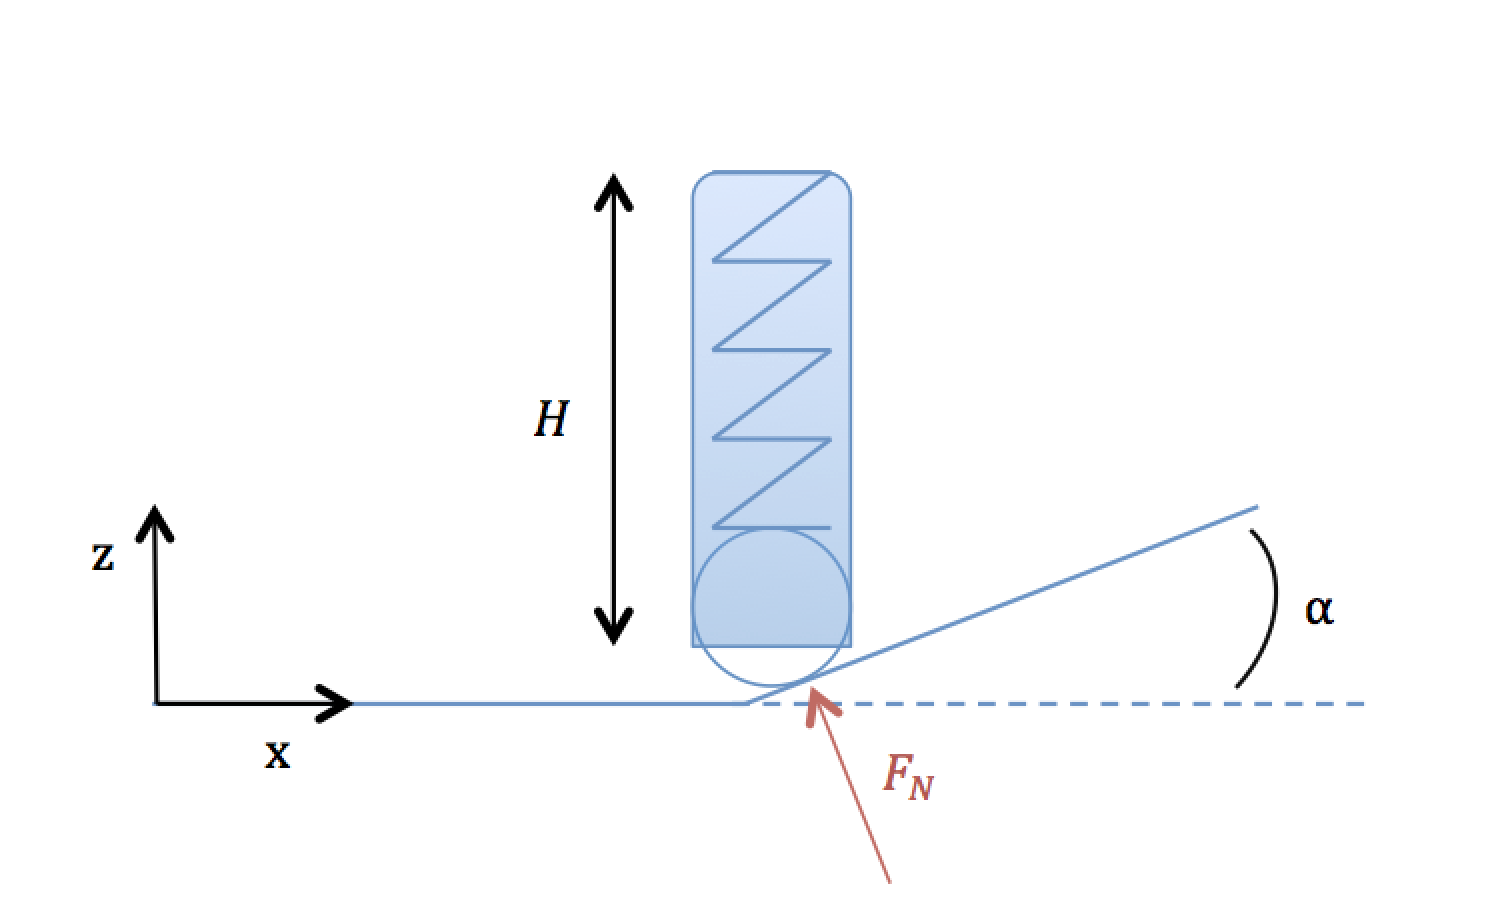
\includegraphics[scale=0.5]{schema_Kalman.png}
\end{center}


\vspace{1cm}
Plaçons nous dans le cas où l'outil n'est plus perpendiculaire à la surface (voir schéma ci-dessus)\\

Etant donné qu'il n'est pas possible de changer l'orientation du robot XXX -> CARO, nous nous bornerons toujours à corriger la trajectoire du robot. \\

\vspace{1cm}
Les valeurs mesurées par le capteur dépendent désormais de l'angle $\alpha$ formé avec l'horizontale. On a 

$$
\begin{array}{lllll}
F_x &=& F_N \sin(\alpha) &\\
F_z &=& F_N \cos(\alpha) &\\
M_y &= &F_x*H & \text{en faisant l'hypothèse que la hauteur découverte de la bille} \\ 
	&&& \text{est négligeable devant la hauteur du poussoir} \\
	&= &F_N \sin(\alpha)*H &
	\begin{array}[t]{l}
	
	\end{array}
\end{array}
$$

L'objectif force devant désormais être mesuré selon la nouvelle normale à la surface, il convient de corriger la matrice D de l'équation de mesure.
On détermine tout d'abord $\alpha$ grâce aux données du capteur:
$$ \alpha = \arctan(\frac{F_{x}}{F_{z}}) $$
On a 
$$
\begin{array}{lll}
F_{z} = k \delta z + F_{obj} cos(\alpha)
\end{array}
$$

soit 
$$
\begin{array}{lll}
D &=& \begin{pmatrix} 0 & \cos(\alpha) \end{pmatrix} \\ 
\end{array}
$$

Afin de tenir compte de la pente imprévue, il faut également ajuster le déplacement et la vitesse selon z. \\
Pour cela, on prend désormais en compte un vecteur commande u correspondant à la vitesse du robot. Afin de suivre la pente, on souhaite désormais imposer une vitesse verticale supplémentaire égale à $\sin{\alpha}*\dot{z}_{robot}$. \\
On pose donc
$$ 
\begin{array}{lll}
u &=& \begin{pmatrix} \dot{z}_{robot} \\ F_{obj}\end{pmatrix} \\
B &=& \begin{pmatrix}	\sin(\alpha) & 0 \\ 0 & 0  \end{pmatrix} \rule{0pt}{20pt}\\
\end{array}
$$



\noindent Les matrices V et W sont modifiées car une nouvelle source d'imprécision est apporté par l'introduction du paramètre alpha. 


\subsection{Modèle 2D avec prise en compte du frottement}








\end{document}